\documentclass[tikz]{standalone}
\usepackage{tikz}
\begin{document}
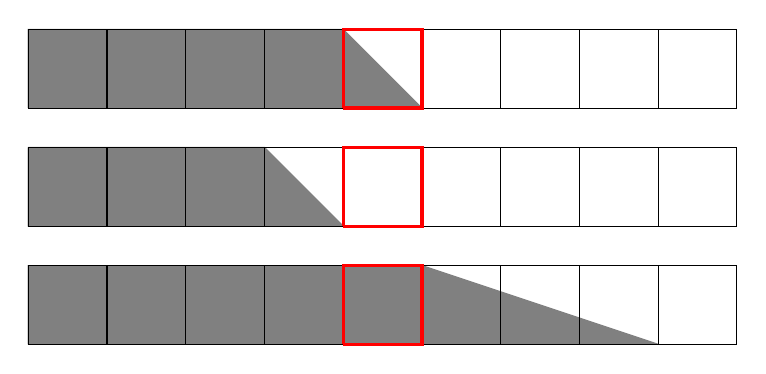
\begin{tikzpicture}
  \begin{scope}[scale=1]
    \filldraw[gray] (-4.0,0)--(1.0,0)--(0,1)--(-4.0,1)--(-4.0,0);
    \draw[step=1cm] (-4.0,0) grid (5.0,1.0);
    \draw[very thick,red] (0,0)--(0,1)--(1,1)--(1,0)--(0,0);
  \end{scope}
  \begin{scope}[scale=1,yshift=-1.5cm]
    \filldraw[gray] (-4.0,1)--(-1,1)--(0,0)--(-4.0,0)--(-4.0,1);
    \draw[step=1cm] (-4.0,0) grid (5.0,1.0);
    \draw[very thick,red] (0,0)--(0,1)--(1,1)--(1,0)--(0,0);
  \end{scope}
  \begin{scope}[scale=1,yshift=-3cm]
    \filldraw[gray] (-4.0,0)--(4.0,0)--(1.0,1)--(-4.0,1)--(-4.0,0);
    \draw[step=1cm] (-4.0,0) grid (5.0,1.0);
    \draw[very thick,red] (0,0)--(0,1)--(1,1)--(1,0)--(0,0);
  \end{scope}
\end{tikzpicture}
\end{document}
